\documentclass{article}[16pt]
\usepackage[utf8]{inputenc}

\usepackage[utf8]{inputenc}
\usepackage[russian]{babel}
\usepackage{geometry}
\usepackage{amsmath}
\usepackage{amsthm}
\usepackage{amssymb}
\usepackage{fancyhdr}
\usepackage{setspace}
\usepackage{graphicx}
\usepackage{colortbl}
\usepackage{tikz}
\usepackage{pgf}
\usepackage{subcaption}
\usepackage{listings}
\usepackage[colorlinks, linkcolor=blue, urlcolor=blue]{hyperref}
\usepackage{indentfirst}
\usepackage{float}
\usepackage{wrapfig}
\graphicspath{{images/}}


\makeatletter
\renewcommand{\@biblabel}[1]{#1.} 
\makeatother

\geometry{left=2.5cm}
\geometry{right=1.5cm}
\geometry{top=1.5cm}
\geometry{bottom=1.5cm}
\renewcommand{\baselinestretch}{1.5}

\newcommand{\bibref}[3]{\hyperlink{#1}{#2 (#3)}}

\title{Прямая оптимизация метрик ранжирования. \\Проект по курсу Машинное обучение \\Отчет}
\author{Семененя Яна Игоревна БПМИ172 \\ Кузнецов Дмитрий Сергеевич БПМИ171}
\date{Май 2020}

\begin{document}
\maketitle

\newpage
\textbf{Ссылка на исходный код проекта -} \bibref{source}{Semenenia et al.}{2020}

\section{Описание задачи.}

Целью задачи ранжирования является задание определенного порядка на множестве объектов.  Обучение ранжированию представляет собой следующую задачу. Пусть дано множество объектов $\mathbb{X}$ и обучающая выборка $X = (x_1,...,x_n) \subset \mathbb{X}$ для которой известен некоторый порядок. То есть целевая переменая представляет собой множество пар $(i, j) \in R \subset (1, ..., n)^2$, где i-й объект в отсортированном списке находится ниже чем j-й объект.
Требуется построить такую модель $a: \mathbb{X} \to R$, что для $(i, j) \in R$ выполнено $a(x_i) < a(x_j)$.

Существует несколько подходов к решению данной задачи. Мы рассмотрим pairwise и listwise подходы. В парном подходе задача обучения формализуется как классификация пар объектов на две категории: правильно ранжированные и неправильно ранжированные.
То есть задача ранжирования в попарном подходе сводится к оптимизации следующего функционала ошибки:
$$\sum\limits_{(i,j) \in R} [a(x_j) - a(x_i)] < 0$$ 
где R - множество пар, на которых известен порядок. 

В списочных методах на вход модели подаются сразу все объекты, а на выходе мы получаем их перестановку. Целью обучения для таких методов является минимизация следующего функуионала ошибки:
$$\sum\limits_{i=1}^n L(a(x_i), y_i)$$
где L - списочная функция потерь. В результате такой постановки задачи списочные методы позволяют напрямую оптимизировать метрики качества ранжирования. Например, в методе AdaRank списочная функция потерь определяется как:
$$L = exp(-NDCG(a(x), y))$$


Далее мы рассмотри различные методы решения задачи ранжирования документов относительно соответствующих запросов.

\section{Описание данных}
\begin{figure}[t]
\centering
\begin{tabular}{ | c | c | c |  }
\hline
	Признак & Формула & Описание  \\ \hline
	L1 & $\sum_{q_i \in q \cap d} c(q_i, d)$ & Частота слова(TF) \\ \hline
	L2 &  $\sum_{q_i \in q \cap d} log(c(q_i, d)+1)$ & Признак из SIGIR статьи \bibref{arsvm}{Cao et al.}{2006} \\ \hline
	L3 & $\sum_{q_i \in q \cap d} \frac{c(q_i,d)}{|d|}$ & Нормализованный TF \\ \hline
	L4 & $\sum_{q_i \in q \cap d} log\left(\frac{c(q_i,d)}{|d|} + 1\right)$ & Признак из SIGIR статьи \\ \hline
	L5 & $\sum_{q_i \in q \cap d} log\left(\frac{|C|}{df(q_i)}\right)$ & IDF \\ \hline
	L6 & $\sum_{q_i \in q \cap d} log(log(\frac{|C|}{df(q_i)}))$ & Признак из SIGIR статьи \\ \hline
	L7 & $\sum_{q_i \in q \cap d} log\left(\frac{|C|}{c(q_i, C)} + 1\right)$ & Признак из SIGIR статьи \\ \hline
	L8 & $\sum_{q_i \in q \cap d} log\left(\frac{c(q_i,d)}{|d|} log(\frac{|C|}{df(q_i)})+1\right)$ & Признак из SIGIR статьи \\ \hline
	L9 & $\sum_{q_i \in q \cap d} c(q_i,d)log \left(\frac{|C|}{df(q_i)}\right)$ & TF*IDF \\ \hline
	L10 & $\sum_{q_i \in q \cap d} log \left(\frac{c(q_i, d)}{|d|} \frac{|C|}{c(q_i, C)} + 1 \right)$ & Признак из SIGIR статьи \\
	\hline
\end{tabular}
\caption{Таблица признаков и их описание} \label{table:features}
\end{figure}

В данном исследовании мы использовали набор данных OHSUMED, представленный в LETOR 1.0 \bibref{letor}{Qin et al.}{2009}. Данные содержат 106 запросов, соответствующие поиску медицинских публикаций. С каждым запросом связано некоторое количество документов. Всего данные сожердат 16140 пар запросов-документ.
Каждые пара запрос-документ представляет из себя объект из 25 признаков. Из заголовков и аннотаций статей были получены по 10 признаков с помощью формул из таблицы \ref{table:features}.Еще 5 были получены с помощью их комбинаций.


\section{Описание метрик}
	В данном разделе мы опишем метрики, использующиеся в задаче ранжирования. Мы не будем рассматривать классические метрики машинного обучения (в частности, $F-score$), которые могут использоваться, например, в pairwise-методах.
	
	Пусть $q$ некоторый запрос и $x = (x_1, \dots, x_n)$ документы, соответствующие этому запросу. Не умоляя общности, пусть $a$ - некоторый алгоритм, выдающий меру релевантности для документа ($>0$ - документ релевантен, больше мера - документ более релевантен). Пусть $y = (y_1, \dots, y_n)$ истинные релевантности документов ($>0$ - документ релевантен запросу).
	
	Введем следующие метрики.
	
	\subsection{Precision at k}
	\begin{equation}
		precisio@k(q) := \frac{\{x_i \in x | ~ a(x_i) > 0 ~ \& ~ y_i > 0\}}{\{x_i | a(x_i) > 0\}}
	\end{equation}

	Данная метрика равна доле действительно релевантных документов среди документов, которые наша модель пометила как релевантные.
	
	\subsection{Average precision at k. MAP}
	\begin{equation}
		AP@k(q) := \sum_{i=1}^{k} \frac{y_{(i)}}{\sum_{j=1}^{k}y_{(j)}}precision@i(q)
	\end{equation}
	
	Здесь $y_{(i)}$ - i-ая порядковая статистика. Метрика равна выпуклой комбинации precision`ов от топ $k$ позиций. 
	
	Данную метрику можно продолжить на всю выборку и ввести:
	\begin{equation}
		MAP@k(a, \mathbf{Q}) := \frac1{|\mathbf{Q}|}\sum_{q \in \mathbf{Q}} AP@k(q)
	\end{equation}
	
	\subsection{Discounted Cumulative Gain. nDCG}
	\begin{equation}
		DCG@k(q) := \sum_{i=1}^{k} g(y_{(i)}) \, d(i)
	\end{equation}
	
	Здесь, $g$ - некоторая функция награды за ранжирования, а $d$ - штраф за позицию. В нашей работе мы использовали следующие функции:
	\begin{equation*}
		g(y) := 2^y - 1
	\end{equation*}
	\begin{equation*}
		d(i) := \frac1{\log_2 (i + 1)}
	\end{equation*}
	
	Поскольку $DCG$ сложно интерпретировать, можно ввести отнормированный на идеальное ранжирование аналог:
	\begin{equation}
		nDCG@k(q) := \frac{DCG@k(q, a)}{\max_{\hat{a}} DCG@k(q, \hat{a})}
	\end{equation}
	
	\subsection{Mean Reciprocal Rank}
	\begin{equation}
		MRR(\mathbf{Q}) := \frac1{|\mathbf{Q}|}\sum_{q \in \mathbf{Q}} rank_q
	\end{equation}
	
	Здесь $rank_q$ - позиция первого релевантного документа в ранжировании запроса $q$.
	\section{Цель данной работы}
	В отличие от классических метрик, метрики ранжирования более интерпретируемы и коррелирует с реальным качеством модели ранжирования. По этой причине конечной мерой качества служит одна из выше описанных метрик (есть и другие, но в контексте наших данных они плохо применимы). Для нас было бы более предпочтительным напрямую оптимизировать метрики, которые описывают конечное качество модели. К сожалению, рассмотренные функции не являются дифференцируемыми по параметрам модели, и, как следствие, мы вынуждены использовать pairwise-подход, в котором оптимизируются некоторый другой функционал, коррелирующий с данными. Тем не менее, существуют и другие подходы к разрешению проблемы дифференцируемости метрик.
	
	В данной работе мы хотим рассмотреть подходы, которые оптимизируют напрямую метрики ранжирования. Сравнить их с одним из pairwise-методов.
	
	\section{Описание методов}
	Во всех разделах кроме RankSVM положим следующую нотацию. (В нем используем нотацию введенную в постановке pairwise-подхода)
	
	$\mathbf{Q} = (q_1, \dots, q_m)$ - множество запросов. $d_i$ - множество документов, выданное по запросу $q_i$ (в частности, $d_{ij}$ - jый среди них). 
	
	$x_{ij}$ - векторное описание jго документа для запроса $q_i$. 
	
	$y_{ij}$ - истинная мера релевантности, соответствующая $j$му документу для запроса $q_i$
	\subsection{Baseline. RankSVM}
	В качестве baseline мы рассмотрим pairwise-метод: RankSVM. Выбор остановили на нем, т.к. в статьях среди pairwise-подходов он зарабатывает одни из лучших результатов.
	
	Как и всякий pairwise, RankSVM оптимизирует (не напрямую) следующий функционал:
	\begin{equation*}
		\sum_{(i, j) \in R} [a(x_j) - a(x_i) < 0] \rightarrow \min
	\end{equation*}
	
	Зная условную задачи оптимизации SVM, отсюда несложно получить условную задачу оптимизации данного функционала для SVM:
	\begin{equation}
		\begin{cases}
		\frac12 ||w||^2 + C \sum_{(i, j) \in R} \xi_{ij} \rightarrow \min_{w, \xi} \\
		w^T(x_j - x_i) \ge 1 - \xi_{ij}, & (i, j) \in R \\
		\xi_{ij} \ge 0, & (i, j) \in R
		\end{cases}
	\end{equation}
	
	В силу линейности модели, данный подход не требует особой имплементации. Достаточно преобразовать pairwise-данные к виду $\hat{\mathbf{X}} = \{x_j - x_i\}_{(i, j) \in R}$ и ввести лэйблы для обучения: $\hat{y} = \{1\}_{(i, j) \in R}$.
	
	В такой постановке обучение классического SVM будет эквивалентен оптимизации задачи (7).
	
	\subsection{AdaRank}
	Первый из рассмотренных методов прямой оптимизации метрик ранжирования - AdaRank от \bibref{adaRank}{Xu et al.}{2007}. 
	
	Данный подход определяет оптимизируемую метрику $E(\pi(q, d, f), y)$, зависящую от некоторой перестановки документов внутри запроса $q$ с точки зрения модели. В частности, в качестве такой метрики и выступает либо $nDCG$, либо $MAP$.
	
	Напомним, что итоговый алгоритм определяется следующим образом:
	\begin{equation}
		f_t(x) = \sum_{k=1}^t \alpha_k h_k(x)
	\end{equation}
	где $h_k$ базовый алгоритм бустинга (в частности, постоянные функции).
	
	AdaRank отличается от родительского метода AdaBoost выбором весов моделей и объектов. В данном методе они определяются по следующему правилу:
	\begin{equation}
		\alpha_t = \ln \frac{\sum_{i=1}^m P_t(i) [1 + E(\pi (q_i, d_i, h_t), y_i)]}{\sum_{i=1}^m P_t(i) [1 - E(\pi (q_i, d_i, h_t), y_i)]}
	\end{equation}
	
	\begin{equation}
		P_{t+1}(i) = \frac{\exp[-E(\pi (q_i, d_i, f_t), y_i)]}{\sum_{j=1}^m exp[E(\pi (q_j, d_j, h_t), y_j)]}
	\end{equation}
	
	Предсказания строятся: $f(x) = f_T(x)$
	
	В целом, как и в AdaBoost, AdaRank итеративно обновляет веса при объектах таким образом, что вес объекта во время оптимизации тем больше, чем ниже на нем метрика ранжирования. Т.е. чем хуже качество ранжирования на данном запросе, тем выше при нем вес. Учитывая веса, строит базовый алгоритм на каждой итерации. После чего накапливает взвешенную композицию.
	
	\subsection{ListNet}
	Поскольку ListNet \bibref{listnet}{Cao et al.}{2007} подробно обсуждался в лекциях, мы не будем приводить полную постановку метода. В данном разделе мы остановимся только на эвристической постановке, которую использовали в данной работе.
	
	Вместо того, чтобы приближать вероятности перестановок документов для запроса, мы будем приближать вероятность попасть на первую позицию документу $d_{ij}$ для запроса $q_i$. 
	
	Пусть $f(x)$ - наша модель (определим ее чуть позже). 
	
	Тогда уверенность модели, что документ $d_{ij}$ для запроса $q_i$ попадет на первую позицию:
	\begin{equation}
		a(x_{ij}) = \frac{\exp[f(x_{ij})]}{\sum_{k=1}^{n(i)}\exp[f(x_{ik})]}
	\end{equation}
	
	Истинной вероятностью попадания такого документа на первую позицию положим:
	\begin{equation}
		p(x_{ij}) = \frac{\exp[y_{ij}]}{\sum_{k=1}^{n(i)}\exp[y_{ik}]}
	\end{equation}
	
	Оптимизировать будем cross-entropy этих двух распределений:
	\begin{equation}
		\mathcal{L}(y_i, a_i) = - \sum_{j=1}^{n(i)} p(x_{ij}) \log a(x_{ij})
	\end{equation}
	
	Данный функционал является дифференцируемым по параметрам модели, если сама модель дифференцируема. Более того, мы неявно оптимизируем $nDCG$ (придумали упрощающую эвристику).
	
	В качестве модели положим линейную (стакали слои, работало на порядок хуже):
	\begin{equation}
		f(x) := w^Tx
	\end{equation}

	\begin{flushright}
		\textbf{см. следующую страницу}
	\end{flushright}
	
	\subsection{DirectRanker}
	\begin{figure}[H]
		\centering
		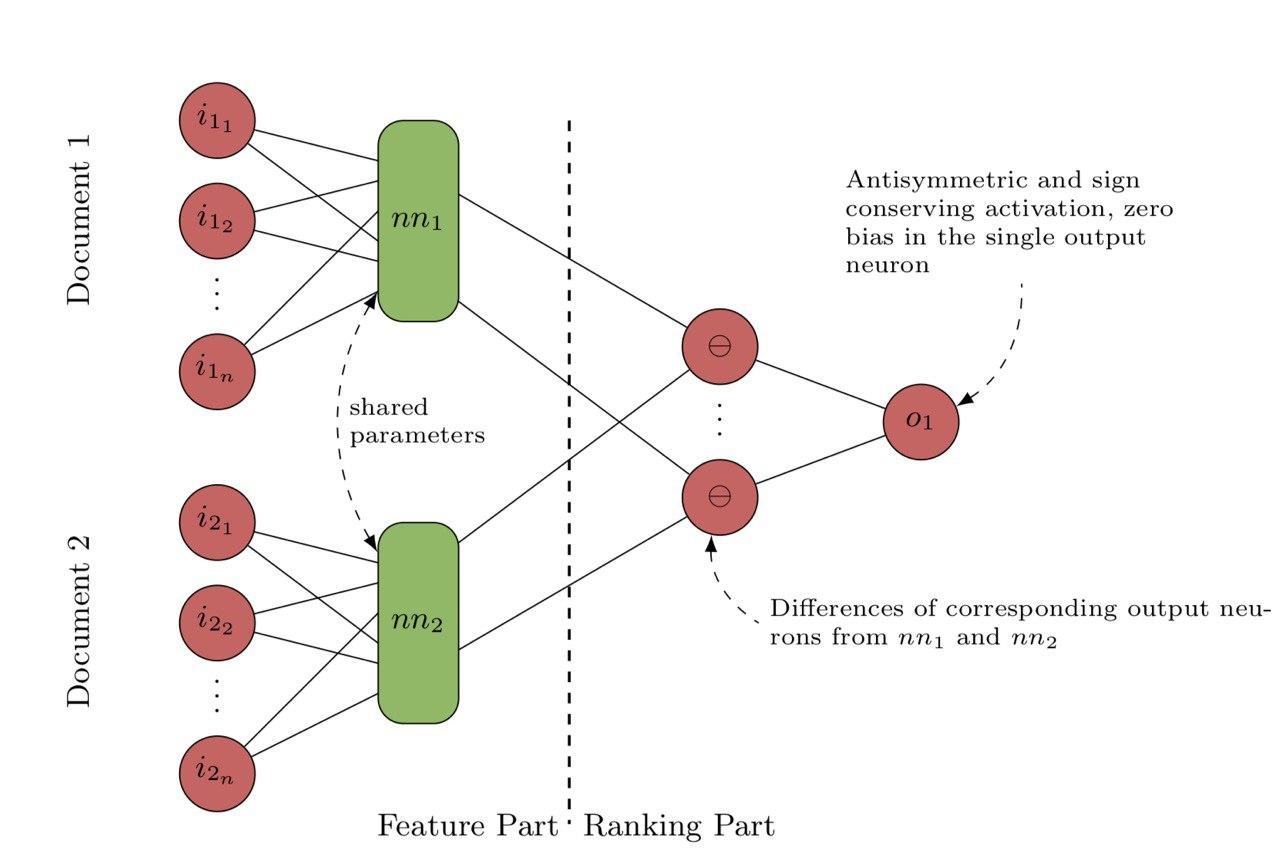
\includegraphics[width=\textwidth]{DirectRanker.png}
	\caption{Схема метода DirectRanker} \label{fig:ranker}
	\end{figure}
	
	DirectRanker относится к парному методу. Схема этого метода приведена на рис. \ref{fig:ranker} \bibref{last}{Koppel et al.}{2019}.

	На приведенной схеме $nn_1$ и $nn_2$ могут быть произвольными сетями, которые для одинаковых документов i и j, дают одинаковый выход. Эти сети должны быть идентичными, то есть иметь одинаковую структуру и параметры, такие как веса, смещения и функции активации. Разница выходов подсетей подается в третью подсеть, которая состоит только из одного выходного нейрона с антисимметричной активацией, сохраняющей знак. Оптимизируемый функционал в данном методе является свободным задаваемым параметром.
	В данном эксперименте в качестве сети используется двухслойная полносвязная сеть, в качестве функции активации взят гиперболический тангенсч, оптимизируемый функционал - кросс-энтропия.

	Авторами статьи показывается, что функция задаваемая данным алгоритмом ранжирования антисимметрична, транзитивна и рефлексивна.
	Антисимметричнось позволяет обучаться только на парах объектов где первый объект менее релевантен чем второй. 
	Транзитивность позволяет не сравнивать совсем не релевантные документы с наиболее релевантными при условии что каждый документ обучается по меньшей мере с помощью документов из соответствующих соседних классах релевантности. 
	Рефлексивность позволяет не обучаться на парах документов с одинаковой релевантностью, что дает оптимизатору больше свободы для поиска оптимального решения для ранжирования.
	\subsection{SVM-MAP}
	Исходный код реализации: \bibref{svmmap_source}{Yue et al.}{2011}
	
	Рассмотрим другую версию SVM: SVM-MAP \bibref{svmmap}{Yue et al.}{2007}. Данный подход на этот раз напрямую оптимизируют метрику ранжирования: MAP. 
	
	Пусть мы хотим построить модель:
	\begin{equation}
		h: \mathbb{X} \rightarrow \mathbb{Y}
	\end{equation}
	
	Пусть у нас определен некоторый лосс:
	\begin{equation}
		\Delta: \mathbb{Y}\times\mathbb{Y} \rightarrow \mathbb{R}
	\end{equation}
	
	Не умоляя общности, определим метод для фиксированного $q$, на случай нескольких запросов, метод легко масштабируется. (Как следствие, будем упускать индекс запроса в обозначениях).
	
	Пусть $C$ - множество релевантных документов, а $\hat{C}$ - множество нерелевантных для запроса документов.
	
	Положим следующую функцию:
	\begin{equation}
		\Psi(x, y) := \frac1{|C||\hat{C}|} \sum_{i:~d_i \in C} \sum_{j: ~d_j \in \hat{C}} [
			sign (y_i - y_j) (x_{i}- x_j)
		]
	\end{equation}
	
	Тогда задача безусловной оптимизации SVM-MAP:
	\begin{equation}
		\begin{cases}	
			\frac12 ||w||^2 + \frac{C}{n}\sum_{i=1}^n \xi_i \rightarrow \min_{w, ~\xi \ge 0} \\
			\forall i \forall y \in \mathbb{Y}:
			w^T\Phi(x_i, y_i) \ge w^T\Phi(x_i, y) + \Delta(y_i, y) - \xi_i
		\end{cases}
	\end{equation}
	
	Причем данная задача минимизирует MAP. 
	
	Тогда наша модель:
	\begin{equation}
		h(x, w) = argmax_{y \in \mathbb{Y}} [w^T\Phi(x, y)]
	\end{equation}

	\section{Эксперименты}
	\subsection{Описание}
	Каждая модель из описанных выше была обучена на датасете OHSUMED. Train составляет $90\%$ от выборки, $10\%$ - test. (Валидация входила в тест).
	
	RankSVM обучался, итеративно решая безусловную задачу оптимизации (7). 
	
	SVM-MAP - (18) минимизируя MAP.
	
	DirectRanker - cross-entropy.
	
	Остальные методы оптимизировали $nDCG$.
	
	Далее, все описанные выше метрики, были посчитаны для каждого метода на тестовом множестве.
	
	\subsection{Результаты}
	\begin{figure}[H]
		\begin{subfigure}{.33\textwidth}
			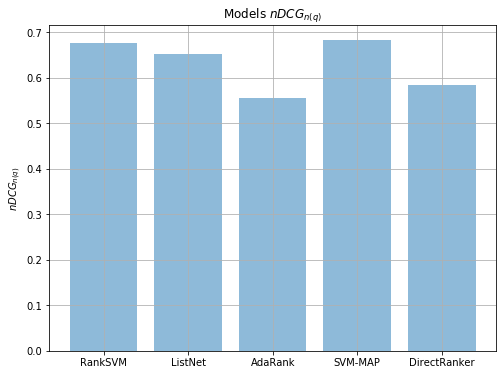
\includegraphics[width=\textwidth]{images/nDcg.png}
			\center{\caption{$nDCG@n$}\label{fig:ndcg}}
		\end{subfigure}
		\begin{subfigure}{.33\textwidth}
			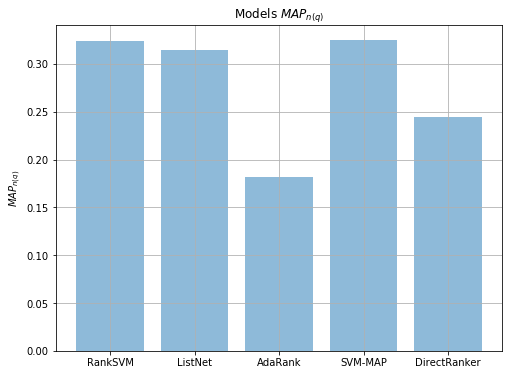
\includegraphics[width=\textwidth]{images/map.png}
			\center{\caption{$MAP@n$}\label{fig:map}}
		\end{subfigure}
		\begin{subfigure}{.33\textwidth}
			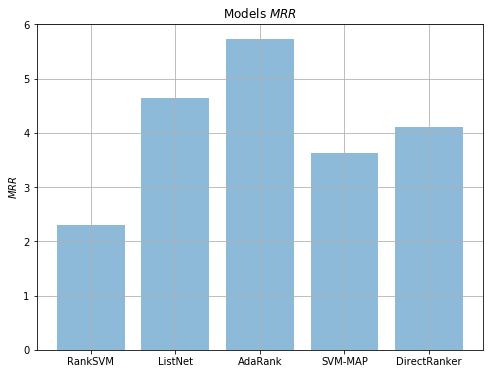
\includegraphics[width=\textwidth]{images/mrr.png}
			\center{\caption{$MRR$}\label{fig:mrr}}
		\end{subfigure}
	\end{figure}
	
	В первую очередь рассмотрим $nDCG$ (рис. \ref{fig:ndcg}). Как видно из графика - явный фаворит - SVM-MAP, чуть хуже работает RankSVM. ListNet работает по качеству в том же порядке, что и эти методы. Однако, AdaRank и, что более удивительно, DirectRanker на порядок хуже, всех других методов. В причинах таких результатов мы постараемся разобраться далее. 
	
	Обращаясь к рис. \ref{fig:map}, можно заметить интересную особенность, относительный порядок методов с точки зрения MAP в точности совпадает с порядком на nDCG. Однако, AdaRank и DirectRanker с точки зрения  MAP отстают еще больше, несмотря на то, что масштаб метрики MAP ниже.
	
	Более неожиданный и менее согласованные результаты можно наблюдать на рис. \ref{fig:mrr}. Как мы видим, фаворит в этом случае - RankSVM, в среднем релевантный документ у него появляется раньше в ранжировании, несмотря на то, что в nDCG он проигрывает SVM-MAP и, более того, не является методом прямой оптимизации. В то же время, ListNet показывает сравнительно более плохие результаты с точки зрения среднего ранга. 
	
	Важной характеристикой моделей является - время работы. RankSVM на предложенных данных тратит наибольшее время на обучение (в зависимости от вычислителя - $\sim 45 min$, в свою очередь - adaRank обучается буквально за секунду. SVM-MAP требует на обучение несколько минут. Остальные методы - имеют сравнимо небольшое время обучения (меньше пары минут).
	
	\subsection{Анализ результатов}
	Ключом к обоснованию полученных результатов является формат рассмотренных данных, а именно дискретность истинных релевантностей. Три худших результата получены методами, которые сильно зависят от распределения таргетов. 
	
	В частности, сами авторы DirectRanker в статье помечают, что в теории метод может работать с дискретными таргетами, однако на практике, зачастую требуется небинарное ранжирование (наш случай, т.к. мы считаем метрики ранжирования), в подобных случаях DirectRanker работает плохо. 
	
	Причина относительно плохих результатов AdaRank и ListNet аналогичная. Лучше всего она визуализируется на ListNet. В момент очередного шага оптимизации мы приближаем распределение модеьных релевантностей к софтмаксу таргетов. Однако, как будет выглядеть софтмакс выборки из элементов $\{0, 1, 2\}$? Очевидно, что будет три кластера одинаковых значений, более того, значения между кластерами не будут сильно различаться. Наша модель разделяет свои веса между запросами, на каждой итерации мы пытаемся обучить релевантности (кот-ые должны по хорошему представлять собой строгий вариационный ряд), используя кусочно-постоянный софтмакс. В итоге мы имеем очень слабо обученную модель, которая не способна качественно ранжировать объекты внутри кластеров похожести. Если анализировать выходы ListNet на тестовом множестве, можно легко заметить эти кластеры одинаковых значений. 
	
	Тем не менее, ListNet достаточно близка к результатам SVMов на метриках $nDCG$ и $MAP$. Однако, очень проседает на $MRR$. Этот феномен легко объяснить аналогичным рассуждениями. Поскольку значения между кластерами одинаковых значений ($0$, $1$) не сильно отличаются, ListNet на первые позицию со схожей вероятностью часто выдает вместо документов с релевантностью $2$, документы с релевантностью $1$, т.к. плохо их различает. В силу нашей реализации $MRR$ (мы считаем ранк по первому документу с релевантностью $2$), отсюда и получаем просадку в $MRR$ у ListNet.
	
	В свою очередь, лучшие результаты заработало семейство SVM-методов. И это тоже показательный результат. Т.к. это два единственных метода, которые не зависят от распределения таргетов (истинных релевантностей), SVM-MAP - требует бинарную категорию (релевантен/нерелевантен), а RankSVM - требует в принципе бинарное отношение на парах, для обоих методов все равно какие значения у истинных релевантностей. По этой причине они зарабатывают на рассмотренных данных наилучшие результаты. В силу того, что SVM-MAP более мощный метод (метод прямой оптимизации), мы и получаем для него более хорошую метрику.
	
	Долгое время обучения RankSVM обусловлено тем, что это pairwise подход, который оптимизируется по многочисленным парам. Более того, в отличие от других подходов, метод (из-за того, что он попарный) требует много лишней памяти, что делает его особенно не предпочтительным по сравнению с SVM-MAP.
	
	\section{Выводы}
	В результате экспериментов, были получены неожиданные и удивительные результаты. Самый мощный и современный метод DirectRank оказался одним из худших на предложенных данных, как и чуть менее мощный - AdaRank. В свою очередь, бейзлайн (самый простой подход)  RankSVM получил одни из лучших результатов по качеству.
	
	Однако, было бы некорректно подводить итоговое ранжирование методов (какой из них лучше/хуже), поскольку, как мы уже выяснили, некоторые методы не достаточно предназначены для работы с теми данными, которые мы рассматривали. Тем не менее, мы можем смело сделать вывод, что из рассмотренных методов в случае дискретных истинных релевантностей стоит однозначно отдавать предпочтение SVM-MAP по всем характеристикам.
	
	В дальнейшем нужно провести аналогичные эксперименты на данных с непрерывными истинными релевантностями, чтобы сделать заключительный вывод.
	
	\begin{thebibliography}{0}
		\bibitem{source}\hypertarget{source}{}
		\href{https://github.com/ElDmitro/Learning2Rank}
		{Semenenia Iana, Kuznetsov Dmitriy. Educational Research Project. Learning to rank metrics direct optimization. 2020}
		\bibitem{adaRank}\hypertarget{adaRank}{}
		\href{http://www.bigdatalab.ac.cn/~junxu/publications/SIGIR2007_AdaRank.pdf}
		{Jun Xu, Hang Li. AdaRank: A Boosting Algorithm for Information Retrieval. SIGIR 2007.}
		\bibitem{listnet}\hypertarget{listnet}{}
		\href{https://www.microsoft.com/en-us/research/wp-content/uploads/2016/02/tr-2007-40.pdf}
		{Zhe Cao, Tie-Yan Liu, Ming-Feng Tsai, Hang Li. Learning to Rank: From Pairwise Approach to Listwise Approach. ICML 2007.}
		\bibitem{svmmap}\hypertarget{svmmap}{}
		\href{https://www.cs.cornell.edu/people/tj/publications/yue_etal_07a.pdf}
		{Yisong Yue, Thomas Finley, Filip Radlinski, Thorsten Joachims. A Support Vector Method for Optimizing Average Precision. SIGIR 2007.}
		\bibitem{svmmap_source}\hypertarget{svmmap_source}{}
		\href{https://www.cs.cornell.edu/people/tj/publications/yue_etal_07a.pdf}
		{Yisong Yue, Thomas Finley, Filip Radlinski, Thorsten Joachims. Implementation: A Support Vector Method for Optimizing Average Precision. 2011.}
		\bibitem{letor}\hypertarget{letor}{}
		\href{https://www.microsoft.com/en-us/research/project/letor-learning-rank-information-retrieval/}
		{Tao Qin Tie-Yan Liu. LETOR: Learning to Rank for Information Retrieval. 2009.}
		\bibitem{arsvm}\hypertarget{arsvm}{}
		\href{https://www.microsoft.com/en-us/research/publication/adapting-ranking-svm-document-retrieval/}
		{Yunbo Cao, Jun Xu, Tie-Yan Liu, Hang Li, Yalou Huang, Hsiao-Wuen Hon. Adapting Ranking SVM to Document Retrieval. 2006.}
		\bibitem{last}\hypertarget{last}{}
		\href{https://arxiv.org/pdf/1909.02768.pdf}
		{Marius Koppel, Alexander Segner, Martin Wagener, Lukas Pensel, Andreas Karwath, Stefan Kramer. Pairwise Learning to Rank by Neural Networks Revisited:Reconstruction, Theoretical Analysis and PracticalPerformance. 2019.}
	\end{thebibliography}

\end{document}